\begin{theo}[Primal Optimization Problem]{Primal}
    We will denote the globally optimal value of the objective function subject to the constraints as the primal optimal value $p^*$, i\@.e\@., 
    \begin{equation*}
        p^* = \left( \min_{x \in \mathbb{R}^n} f(x) \quad \text{s.t.} \quad g(x) = 0 \ \land \ h(x) \geq 0 \right).
    \end{equation*}
    and we will denote this optimization problem as the primal optimization problem.
\end{theo}

\newpage

\begin{theo}[Lagrangian Function and Lagrange Multipliers]{LagrangianFunMultp}
    We define the Lagrangian function to be 
    \begin{align*}
        \mathcal{L}(x, \lambda, \mu) 
            &= f(x) + \sum_{i=1}^l \lambda_i g_i(x) + \sum_{i=1}^m \mu_i h_i(x) \\
            &= f(x) + \lambda^T g(x) + \mu^T h(x).
    \end{align*}
    Here, we have introduced Lagrange multipliers or dual variables $\lambda \in \mathbb{R}^l$ and strictly positive $\mu \in \mathbb{R}^m$. 
\end{theo}

\begin{lem}[Lower Bound Property of Lagrangian]{LowerBoundPrimal}
    If $\tilde{x}$ is a feasible point of (\ref{Primal}) and $\mu \geq 0$, then
    \begin{equation*}
        \mathcal{L}(\tilde{x}, \lambda, \mu) \leq f(\tilde(x)).
    \end{equation*}
    \vspace*{-0.5cm}
\end{lem}

\begin{prf}[Lower Bound Property of Lagrangian]{prfLowerBoundPrimal}
    Since $\tilde{x}$ is feasible, we have $g(\tilde{x}) = 0$ and $h(\tilde{x}) \geq 0$. Therefore, with $\mu \geq 0$, we have:
    \begin{equation*}
        \mathcal{L}(\tilde{x}, \lambda, \mu) = f(\tilde{x}) + \lambda^T \underbrace{g(\tilde{x})}_{=0} + \underbrace{\mu^T}_{\geq 0} \underbrace{h(\tilde{x})}_{\geq 0} \leq f(\tilde{x}).
    \end{equation*}
    \vspace*{-0.5cm}
\end{prf}

\begin{theo}[Lagrange Dual Function]{Dual}
    The Lagrange dual function is defined as the unconstrained infimum of the Lagrangian function over $x$, for fixed multipliers $\lambda$ and $\mu$:
    \begin{equation*}
        q(\lambda, \mu) = \inf_{x \in \mathbb{R}^n} \mathcal{L}(x, \lambda, \mu).
    \end{equation*}
    \vspace*{-0.5cm}
\end{theo}

\begin{lem}[Lower Bound property of Lagrange Dual]{LowerBoundDual}
    If $\mu \geq 0$, then the dual function $q(\lambda, \mu)$ is a lower bound on the primal optimal value $p^*$, i\@.e\@.,
    \begin{equation*}
        q(\lambda, \mu) \leq p^*.
    \end{equation*}
    \vspace*{-0.5cm}
\end{lem}

\begin{prf}[Lower Bound property of Lagrange Dual]{prfLowerBoundDual}
    Since the Lagrange function is bounded from below by Lemma~\ref{LowerBoundPrimal}, we have
    \begin{equation*}
        q(\lambda, \mu) = \inf_{x \in \mathbb{R}^n} \mathcal{L}(x, \lambda, \mu) \leq f(\tilde{x}) \quad \text{for any feasible} \ \tilde{x}.
    \end{equation*}
    Naturally, this inequality holds in particular for the global minimizer $x^*$, which yields:
    \begin{equation*}
        q(\lambda, \mu) \leq f(x^*) = p^*.
    \end{equation*}
    \vspace{-0.7cm}
\end{prf}

\begin{theo}[Concavity of Lagrange Dual]{ConcavityDual}
    The function $q: \ \R^p \times \R^q \rightarrow \R$ is concave, even if the original NLP was not convex. 
\end{theo}

\begin{prf}[Concavity of Lagrange Dual]{prfConcavityDual}
    \vspace*{-0.6cm}
    \begin{minipage}{0.64\textwidth}
        We will show that $-q$ is convex. The Lagrangian $\mathcal{L}$ is an affine function in the multipliers $\lambda$ and $\mu$, which in particular implies that $-\mathcal{L}$ is convex in $\lambda$ and $\mu$. Thus, the function $-q(\lambda,\mu) = \sup_x -\mathcal{L}(x,\lambda,\mu)$ is the supremum of convex functions in $\lambda$ and $\mu$ that are indexed by $x$, and therefore convex.
    \end{minipage}
    \begin{minipage}{0.32\textwidth}
        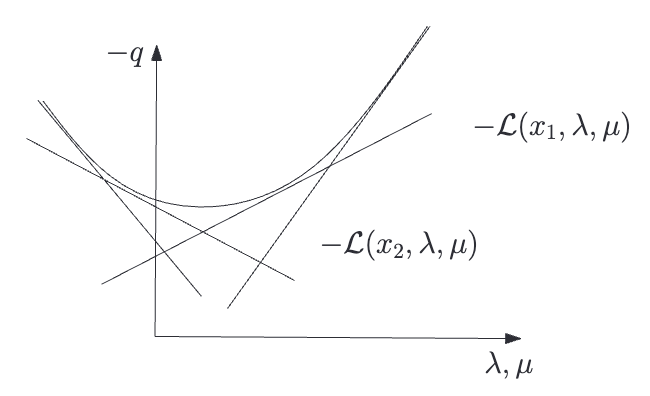
\includegraphics[scale = 0.475]{Images/Fundamental/ConcavityOfDual.png}
    \end{minipage}
    \vspace*{-0.5cm}
\end{prf}

\begin{theo}[Dual Problem]{Dual Problem}
    \vspace*{-0.1cm}
    The dual problem is defined as the convex maximization problem, i\@.e\@.,
    \begin{equation*}
        d^* = \left( \max_{\lambda \in R^p, \mu \in R^q} q(\lambda, \mu) \quad \text{s.t.} \quad \mu \geq 0 \right).
    \end{equation*}
    \vspace*{-0.5cm}
\end{theo}

\begin{theo}[Weak Duality]{Weak Duality}
    \vspace*{-0.1cm}
    Consider a primal-dual pair. Then, the following inequality holds:
    \begin{equation*}
        d^* \leq p^*.
    \end{equation*}
    \vspace*{-0.7cm}
\end{theo}

\begin{theo}[Strong Duality]{Strong Duality}
    \vspace*{-0.1cm}
    If the primal optimization problem is convex and the Slater condition (see Theorem~\ref{Slater}) holds, then strong duality holds, i\@.e\@.,
    \begin{equation*}
        d^* = p^*.
    \end{equation*}
    \vspace{-0.7cm}
\end{theo}

\begin{theo}[Slater Condition]{Slater}    
    If there exist one feasible point $\tilde{x}$ such that all non-linear inequalities are strictly satisfied of a primal convex optimization problem hold, then the Slater condition is satisfied. More explicitly, for a convex problem we must have affine equality constraints, $g(x) = Ax + b$, and the inequality constraint functions can be either affine or concave functions, thus without loss of generality assume that the first $q_1 \leq q$ inequalities are affine and the remaining ones concave. Then the Slater condition holds if and only if there exists an $\tilde{x}$ such that
    \begin{align*}
        A\tilde{x} + b &= 0, \\
        h_i(\tilde{x}) &\geq 0, \quad \text{for} \ i = 1, \ldots, q_1, \\
        g_i(\tilde{x}) &> 0, \quad \text{for} \ i = q_1 + 1, \ldots, q. 
    \end{align*}
    \vspace*{-0.5cm}
\end{theo}
